\documentclass[]{beamer}
%uncomment for notes
%\documentclass[handout]{beamer}
%\setbeameroption{show notes}
%\usepackage{pgfpages}
%\pgfpagesuselayout{4 on 1}[a4paper,border shrink=5mm,landscape]

\graphicspath{{output/}{resources/}}
\DeclareGraphicsExtensions{.pdf,.jpeg,.png,.jpg}
\usepackage[utf8]{inputenc}
\usepackage{epstopdf}
\usepackage{subcaption}
\usepackage{amsmath}
\usepackage{amssymb}
\usepackage[round]{natbib}
\usepackage{tikz}
\usetikzlibrary{fit}
\usetikzlibrary{arrows}
\usetikzlibrary{positioning}

\title{QSAR biodegradation dataset classification using neural networks}
\author{Jonáš Kulhánek, Jan Uhlík}
\institute{MFF, Charles University in Prague}
\date{December 2019}

\usepackage{natbib}
\usepackage{graphicx}
\setbeamertemplate{footline}[frame number]
\setbeamercolor{footline}{fg=blue}
\setbeamerfont{footline}{series=\bfseries}

\begin{document}
\frame[noframenumbering,plain]{
  \titlepage
}
\frame{
  \frametitle{QSAR biodegradation dataset\cite{dataset}}
  \begin{itemize}
    \item Dataset from OpenML: \href{https://www.openml.org/d/1494}{qsar-biodeg}
    \item Classification dataset where the task is to predict whether a protein is bio-degradable based on its chemical properties
    \item Published by Milano Chemometrics and QSAR Research Group
    \item 41 attributes in total, some real valued, other integer valued
    \item Number of proteins in the dataset is 1055
  \end{itemize}
}

\frame{
  \frametitle{Single layer network training}
  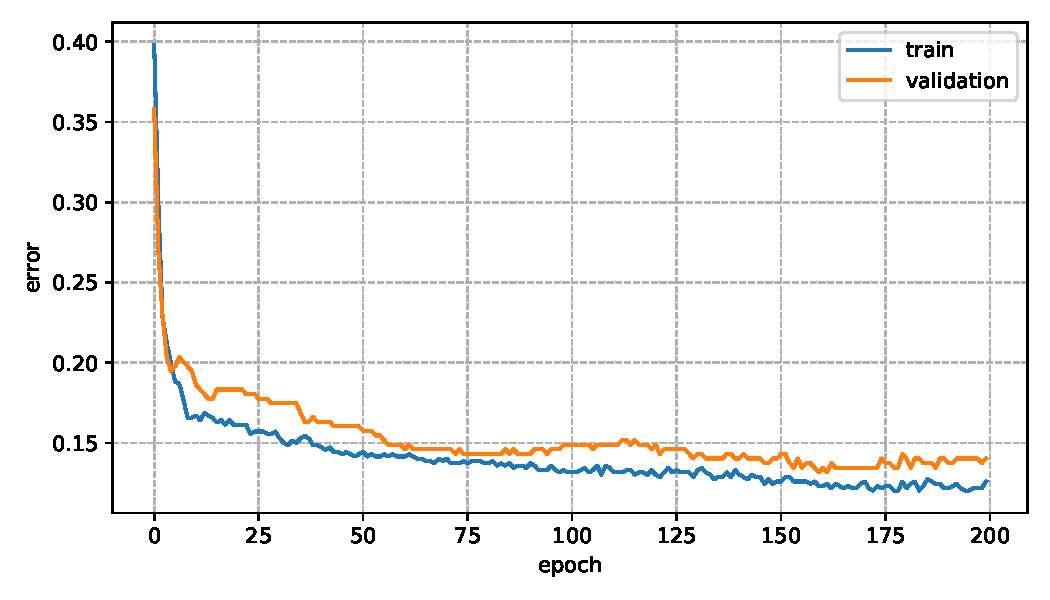
\includegraphics[width=\linewidth]{logreg}
}

\frame{
  \frametitle{Two layers network training}
  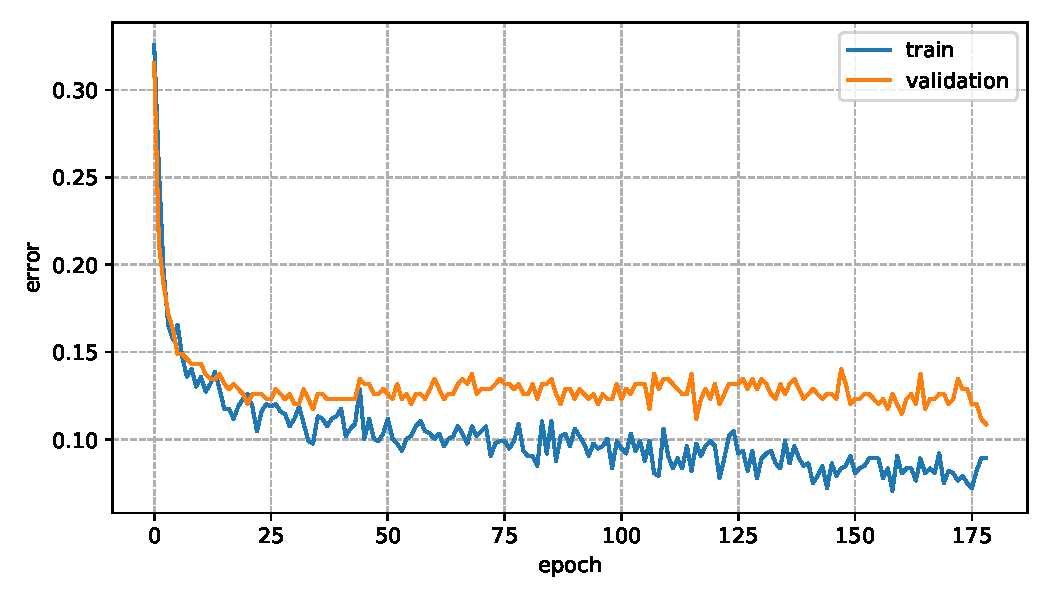
\includegraphics[width=\linewidth]{mlp}
}

\frame{
  \frametitle{Our results and comparisons}
  \begin{table}[]
    \begin{tabular}{|l|l|}
      \hline
      \textbf{Method}                                             & \textbf{Predictive accuracy} \\ \hline
      \texttt{svm.classes.SVC}                   & 89.19\%                      \\ \hline
      \textbf{Ours - 2 layers} & \textbf{89.12\%}             \\ \hline
      \texttt{xgboost}                           & 87.68\%                      \\ \hline
      \texttt{weka.RandomForest}                 & 86.67\%                      \\ \hline
      \textbf{Ours - 1 layer}  & \textbf{85.96\%}             \\ \hline
      \texttt{weka.VotedPerceptron}              & 79.43\%                      \\ \hline
      \texttt{weka.NaiveBayes}                   & 75.64\%                      \\ \hline
      \texttt{neural\_network.MLPClassifier}     & 66.26\%                      \\ \hline
    \end{tabular}
  \end{table}
}

\frame{
  \cite{*}
  \bibliographystyle{plainnat}
  \bibliography{references}
}

\end{document}
